\section{Introduction}


This \cgal\ component implements methods to analyze and process unorganized 3D point sets. The input is an unorganized 3D point set, possibly with attributes such as unoriented or oriented normals. This point set can be analyzed to measure certain geometric properties such as average spacing between the points and their $K$ nearest neighbors. We can furthermore process the point set with functions devoted to the simplification, outlier removal, smoothing, normal estimation and normal orientation. The output is either a point set or a point set with normals.


A typical usage of this package is to pre-process a point set before calling a reconstruction method.


% Insert image introduction.jpg/eps
\begin{center}
    \label{Point_set_processing_3-fig-introduction}
    % Image
    \begin{ccTexOnly}
        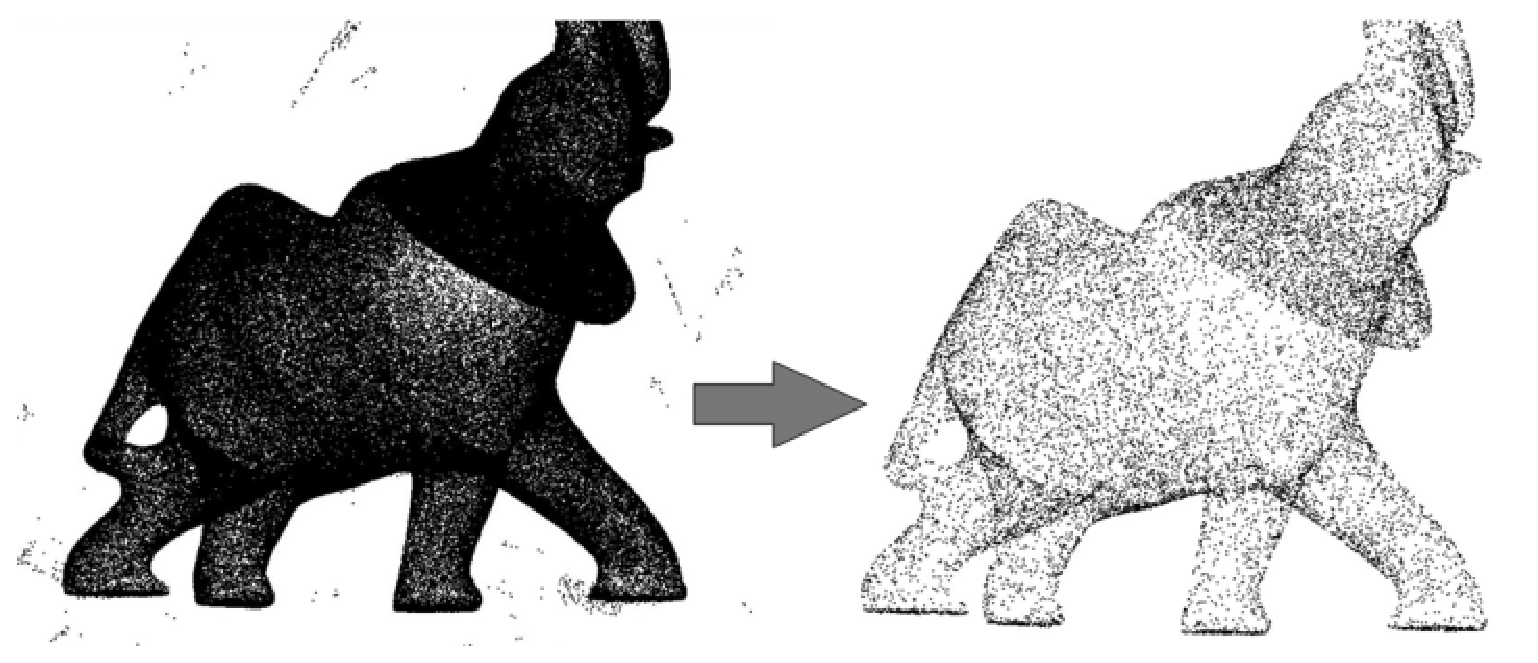
\includegraphics[width=1.0\textwidth]{Point_set_processing_3/introduction} % omit .eps suffix
    \end{ccTexOnly}
    \begin{ccHtmlOnly}
        <img width="90%" border=0 src="./introduction.jpg"><P>
    \end{ccHtmlOnly}
    % Title
    \begin{figure}[h]
        \caption{Point set processing.
                 Left: 275K points sampled on an elephant with
                 a Minolta laser scanner.
                 Right: point set after clean-up and
                 simplification to 17K points.}
    \end{figure}
\end{center}



Surface Reconstruction from Point Sets is a sequential process:

\begin{itemize}
\item Scanning and scan alignment produce a set of points
      or points with normals. Alignment is not yet
      covered by \cgal.
\item Outlier removal for reconstruction methods which
      are not resilient to outliers.
\item Simplification to reduce the number of input points.
\item Smoothing to reduce noise in the input data.
\item Normal estimation and orientation when the normals
      are not already provided by the acquisition device.
\item Surface reconstruction.
\end{itemize}

\cgal\ provides algorithms for all steps listed above except alignment.\\
This package provides outlier removal, simplification, smoothing,
normal estimation and orientation.\\
Chapter \ccc{Surface_reconstruction_points_3} \ref{chap:surface_reconstruction_points_3}
describes surface reconstruction using \cgal\ Surface Mesh Generator.

% Insert image pipeline.jpg/eps
\begin{center}
    \label{Point_set_processing_3-fig-pipeline}
    % Image
    \begin{ccTexOnly}
        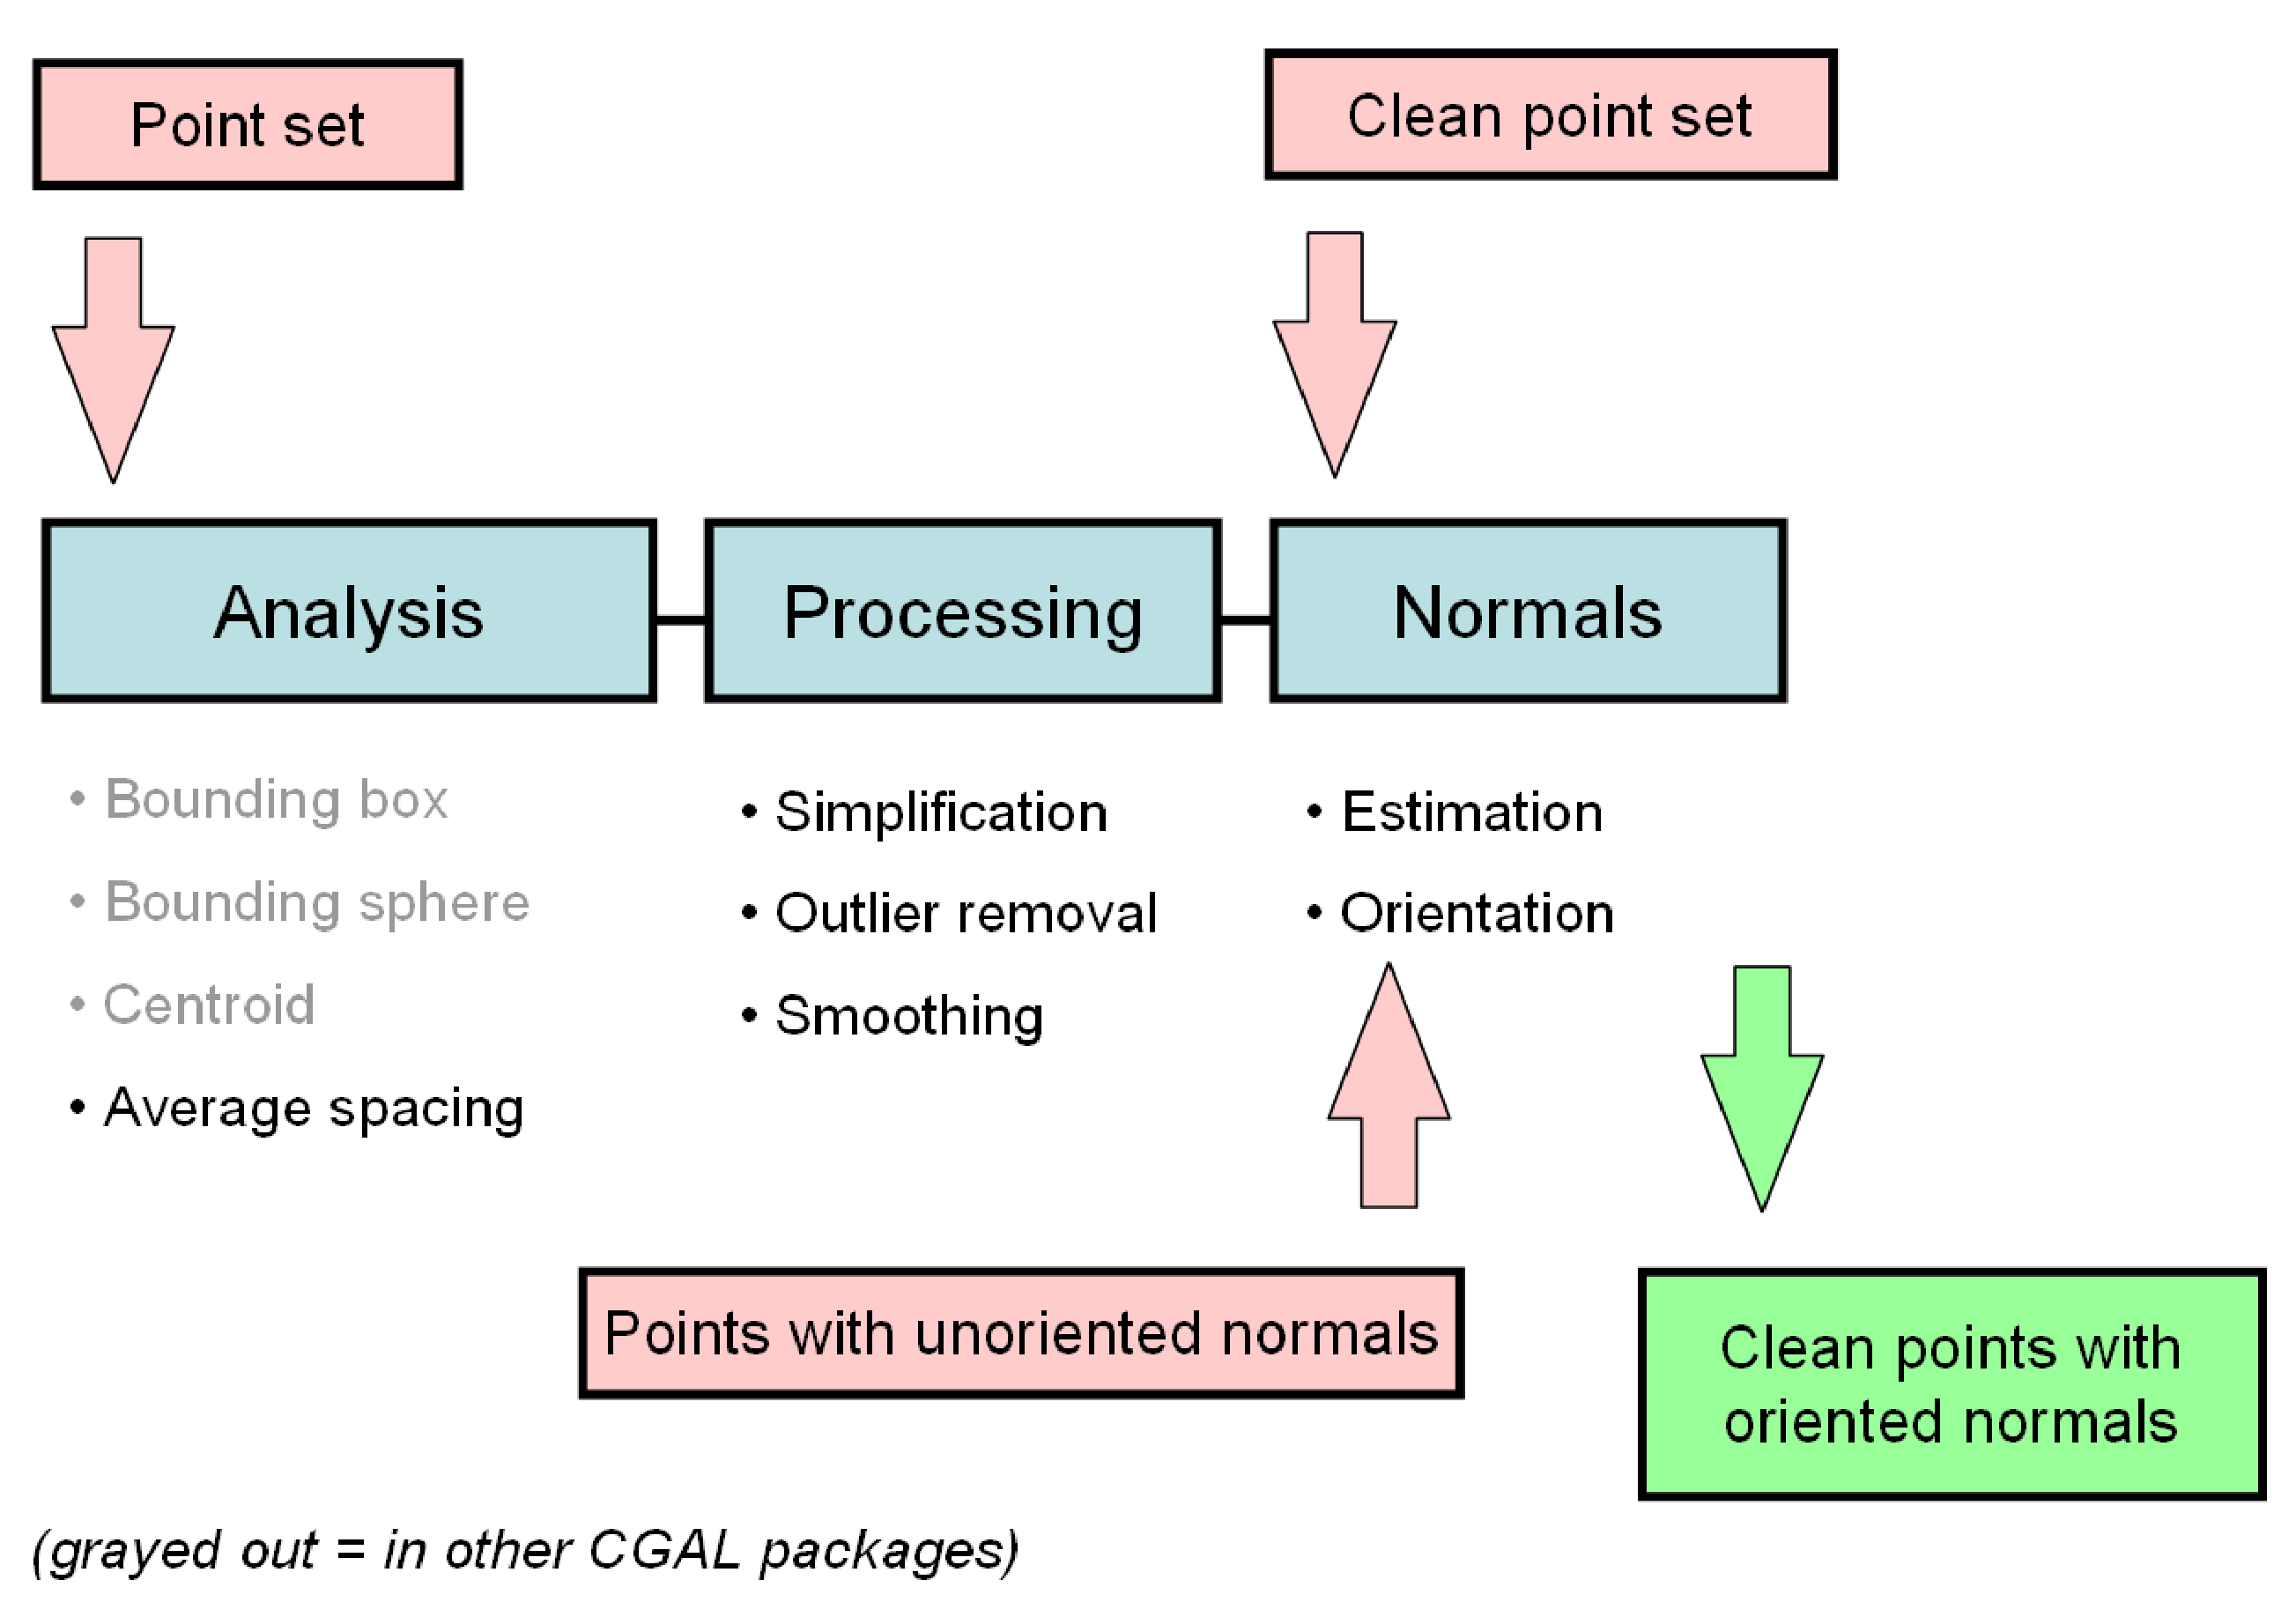
\includegraphics[width=0.8\textwidth]{Point_set_processing_3/pipeline} % omit .eps suffix
    \end{ccTexOnly}
    \begin{ccHtmlOnly}
        <img width="65%" border=0 src="./pipeline.jpg"><P>
    \end{ccHtmlOnly}
    % Title
    \begin{figure}[h]
        \caption{Point Set Processing pipeline.}
    \end{figure}
\end{center}


